\documentclass[11pt,a4paper]{article}

% für \hyphenation mit Umlauten
\usepackage[T1]{fontenc}
\usepackage[utf8]{inputenc}
\usepackage[ngerman,english]{babel}

% Times-Roman-Schrift (auch für mathematische Formeln)
\usepackage{mathptmx} 

% comments
\usepackage{verbatim} 

% Zum Setzen von URLs
\usepackage{color}
\usepackage{alltt}
\definecolor{darkred}{rgb}{.25,0,0}
\definecolor{darkgreen}{rgb}{0,.2,0}
\definecolor{darkmagenta}{rgb}{.2,0,.2}
\definecolor{darkcyan}{rgb}{0,.15,.15}

\usepackage[plainpages=false,bookmarks=true,bookmarksopen=true,colorlinks=true,
  linkcolor=darkred,citecolor=darkgreen,filecolor=darkmagenta,
  menucolor=darkred,urlcolor=darkcyan]{hyperref}

% Zeilenabstand
\renewcommand{\baselinestretch}{1.5}

% anhang
\usepackage[toc,page]{appendix}

% pdflatex: Bilder in den Formaten .jpeg, .png und .pdf
% latex: Bilder im .eps-Format
\usepackage{graphicx}

\usepackage{fancyhdr} % Positionierung der Seitenzahlen
\fancyhead{}
\fancyfoot[C]{\Roman{page}}
\renewcommand{\headrulewidth}{0pt}
\setlength{\headheight}{13.6pt} % behebt headheight Warning

 % behebt headheight Warning
\setlength{\headheight}{13.6pt}

% Korrektes Format für Nummerierung von Abbildungen (figure) und
% Tabellen (table): <Kapitelnummer>.<Abbildungsnummer>
\makeatletter
\@addtoreset{figure}{section}
\renewcommand{\thefigure}{\thesection.\arabic{figure}}
\@addtoreset{table}{section}
\renewcommand{\thetable}{\thesection.\arabic{table}}
\makeatother

% Listings für Sourcecode
\usepackage{listings}
  \usepackage{courier}
 \lstset{
        basicstyle=\footnotesize\ttfamily, % Standardschrift
        numbers=left,               % Ort der Zeilennummern
        numberstyle=\tiny,          % Stil der Zeilennummern
        %stepnumber=2,               % Abstand zwischen den Zeilennummern
        numbersep=5pt,              % Abstand der Nummern zum Text
        tabsize=2,                  % Groesse von Tabs
        extendedchars=true,         %
        breaklines=true,            % Zeilen werden Umgebrochen
        keywordstyle=\color{red},
        frame=b,         
        keywordstyle=[1]{\color{DarkSkyBlue}},    % Stil der Keywords
        keywordstyle=[2]{\color{DarkScarletRed}},    %
        keywordstyle=[3]{\bfseries},    %
        keywordstyle=[4]{\color{DarkPlum}},    %
        keywordstyle=[5]{\color{SkyBlue}},    %
		stringstyle={\color{Chocolate}},
        showspaces=false,           % Leerzeichen anzeigen ?
        showtabs=false,             % Tabs anzeigen ?
        xleftmargin=17pt,
        framexleftmargin=17pt,
        framexrightmargin=5pt,
        framexbottommargin=4pt,
        backgroundcolor=\color{Aluminium1},
        showstringspaces=false,      % Leerzeichen in Strings anzeigen ?
		%language=php
		morekeywords=[1]{Interface,return,static,function}
}
    %\DeclareCaptionFont{blue}{\color{blue}} 

  %\captionsetup[lstlisting]{singlelinecheck=false, labelfont={blue}, textfont={blue}}
  \usepackage{caption}
\DeclareCaptionFont{white}{\color{white}}
\DeclareCaptionFormat{listing}{\colorbox[cmyk]{0.43, 0.35, 0.35,0.01}{\parbox{\textwidth}{\hspace{15pt}#1#2#3}}}
\captionsetup[lstlisting]{format=listing,labelfont=white,textfont=white, singlelinecheck=false, margin=0pt, font={bf,footnotesize}}
\renewcommand\lstlistingname{Codeblock}
 

\sloppy % Damit LaTeX nicht so viel über "overfull hbox" u.Ä. meckert

% Ränder
\addtolength{\topmargin}{-16mm}
\setlength{\oddsidemargin}{40mm}
\setlength{\evensidemargin}{40mm}
\addtolength{\oddsidemargin}{-1in}
\addtolength{\evensidemargin}{-1in}
\setlength{\textwidth}{13cm}
\addtolength{\textheight}{34mm}
%______________________________________________________________________

\hypersetup{
	pdfauthor = {Franziskus Domig, BSc;
		Stefan Gassner, BSc; Wolfgang Halbeisen,
		BSc; Matthias Schmid, BSc},
	pdftitle = {Projekt Dokumentation Roadrunner},
	pdfkeywords = {Roadrunner, Dokumentation, Transport, Logistik},
}

%======================================================================
%
%      Document
%
%======================================================================

\begin{document}

\selectlanguage{ngerman}

\pagestyle{empty} % Vorerst keine Seitenzahlen
\pagenumbering{alpha} % Unsichtbare alphabetische Nummerierung

\begin{center}
\textsc{Fachhochschule Vorarlberg GmbH}\\

\vspace{5cm}
{\large\textbf{Dokumentation}}\vspace{.5cm}

{\LARGE Roadrunner}

\end{center}

\vspace{14cm}


\begin{tabular}{ll}
Projektteam: & Franziskus Domig, Bsc; Stefan Gassner, BSc;\\
	     & Wolfgang Halbeisen, BSc; Matthias Schmid, BSc\\
Bearbeitung: & Dornbirn, im Sommersemester 2011\\
Betreuer:    & Prof.(FH) DI Wolfgang Auer\\
\end{tabular}

%______________________________________________________________________

\clearpage
\pagestyle{fancy}
\pagenumbering{roman} % Römische Seitenzahlen
\setcounter{page}{1}

\tableofcontents


\clearpage
\pagenumbering{arabic}
\setcounter{page}{1}
% Geändertes Format für Seitenränder, arabische Seitenzahlen
\fancyfoot[CO]{\thepage}

\input{input/preface}

\clearpage
\input{input/general}

\clearpage
\input{input/technology}

\clearpage
\section{Datenbank}

Bei einem Überwachungssystem für Warentransporte werden sehr viele Daten entstehen. Diese Daten gilt es zu Verwalten und deren Integrität sicherzustellen. In diesem Kapitel werden unterschiedliche Möglichkeiten der Datenverwaltung betrachtet und erläutert welches System für das Projekt Roadrunner verwendet wird.

\subsection{Datenbankinstanzen}

Anfallende Daten müssen persistent gespeichert werden. Diese Speicherung wird in eine Datenbank durchgeführt. Genauer betrachtet werden die Daten in einer Instanz einer Datenbank gespeichert. Es gilt zu unterscheiden ob eine Instanz einer Datenbank verwendet wird oder mehrere Instanzen verwendet werden und diese synchron gehalten werden.

\begin{description}
	\item[Eine Instanz] Bei der Verwendung einer Datenbankinstanz gibt es einen zentralen Datenbankserver. Alle Daten werden von dieser Instanz gelesen und geschrieben. Der Vorteil dabei ist, dass alle gespeicherten Daten auf dieser Instanz sofort zur Verfügung stehen. Der Nachteil ist, dass die Datenbank für alle Clients durchgehend zur Verfügung stehen muss.
	\item[Mehrere Instanzen - Jeder synchronisiert mit jedem] Wenn mehrere Instanzen einer Datenbank verwendet werden gilt es diese synchron zu halten. Dies bedeutet, wenn auf einer Instanz Daten erzeugt werden, müssen diese mit anderen Instanzen synchronisiert werden. Eine Möglichkeit ist, dass jede Instanz mit allen anderen Instanzen synchronisiert wird. Dies wäre eine Lösung, wenn es eine definierte Menge von Instanzen gibt und jede Instanz von jeder Instanz aus erreicht werden kann. Dadurch ergibt sich Fehlertoleranz gegenüber Ausfällen von einzelnen Datenbankinstanzen, da die Daten auf jeder Instanz vorliegen und es keine zentrale Masterinstanz gibt.
	\item [Mehrere Instanzen - Jeder synchronisiert mit der Masterinstanz] Anstatt dass jede Instanz mit jeder anderen Instanz synchronisiert wird kann auch eine zentrale Masterinstanz verwendet werden. Diese zentrale Instanz hält alle Daten und verteilt diese Daten wenn nötig auf andere Instanzen. Diese bedeutet wenn eine Clientinstanz neue Daten generiert hat werden diese zur Masterinstanz gesendet und wenn der Client bestimmte Daten benötigt kann er diese bei der Masterinstanz abholen. Dadurch ergibt sich aber ein zentraler Fehlerpunkt. Wenn die Masterinstanz ausfällt ist keine Datenverteilung mehr möglich. 
\end{description}

Da beim Roadrunner-Projekt die Daten auf mobilen Geräten erzeugt werden und diese oft auch offline arbeiten, müssen die Daten auf dem Gerät ebenfalls gespeichert werden. Diese Daten werden auf dem Gerät in einer Datenbankinstanz gespeichert. Da es einem mobilen Gerät nicht möglich ist zu allen anderen mobilen Geräten im System Kontakt aufzunehmen wird eine zentrale Masterinstanz verwendet. Auf ein mobiles Gerät werden nur solche Daten gespeichert, die für die Abwicklung der Lieferaufträge benötigt werden.

\subsection{Datenspeicherung}

Daten können in einer Datenbank auf unterschiedliche Arten gespeichert werden. Dieser Abschnitt beschreibt die unterschiedlichen Speicherungsarten und beschreibt ob diese für das Projekt Roadrunner verwendet werden können.

\begin{description}
	\item[Relationale Datenbank] In einer relationalen Datenbank werden Daten in einer Tabelle gespeichert. Tabellen werden über PrimaryKey-ForeignKey-Verknüpfungen miteinander in Verbindung gebracht. Ein Eintrag in eine Tabelle, die auf eine andere Tabelle verweist, kann nur durchgeführt werden wenn der Eintrag auf den verweisen wird in der anderen Tabelle existiert. Somit müssten sehr viele Daten auf die mobilen Geräte verteilt werden. Ein Beispiel: Ein Temperatur-Log-Eintrag gehört zu einem Sensor und zu einem Warengut. Das Warengut befindet sich in einem Transportbehälter und muss somit mit diesem Verknüpft werden. Der Transportbehälter hat ein Fahrzeug. Ein Fahrzeug gehört zu einem Fuhrpark usw. Die Verwendung einer relationalen Datenbank auf einem mobilen Gerät wäre nur möglich wenn unterschiedliche Datenbankschemas für die Instanzen der mobilen Geräte und des Masters verwendet werden. 
	\item[Objektorientierte Datenbank] Die Daten werden direkt als Objekte in die Datenbank gespeichert. Da auf den mobilen Geräten aber Java-Objekte bestehen und auf der Webapplikation PHP-Objekte verwendet werden ist diese Lösung nicht ohne intensiven Programmieraufwand für die Konvertierung möglich.
	\item[Dokumentdatenbank] Die Daten werden als Dokumente in die Datenbank gespeichert. Ein Log-Eintrag ist ein Beispiel solch eines Dokumentes. Dokumente sind für sich unabhängige Datensätze die beliebig in einem System verteilt werden können. Dokumente haben Versionsnummern. Anhand der Versionsnummer erkennt eine Datenbankinstanz ob es eine alte Version eines Dokumentes besitzt und kann bei der Masterinstanz eine neue Version des Dokumentes abholen.
\end{description}

Bei Roadrunner wird eine verteilte Dokumentdatenbank verwendet. Die verwendete Datenbank verwendet als Dokumentstruktur JSON. Für JSON gibt es eine hohe Integration in Java und PHP und ist somit eine einfach zu verwendende Datenstruktur.

\subsection{Datenverteilung}

Daten können auf unterschiedliche Arten im System verteilt werden. Eine Möglichkeit wäre die Daten aus der mobilen Datenbankinstanz in die Applikation zu lesen und das Senden der Daten an die Masterinstanz über die Applikation durchzuführen. Eine andere Möglichkeit ist es, die Datenbanksynchronisierung direkt von den Datenbanken durchführen zu lassen. 

Bei der verwendeten Datenbank im Roadrunner-Projekt wird die Synchronisierung der Daten von den Datenbankinstanzen durchgeführt. Diese Synchronisierung nennt sich Replizierung und es kann dabei angegeben werden welche Daten synchronisiert werden sollen.

\subsection{CouchDB}

Dieser Abschnitt beschreibt wie CouchDB die Anforderungen erfüllt.

\subsection{Alternative Datenbanksysteme}

Dieser Abschnitt beschreibt die möglichen alternativen Datenbanksysteme (z.B. Cassandra) und warum CouchDB als Datenbanksystem ausgewählt wurde.


\clearpage
\section{CouchDB}

\subsection{JSON}

Als Dokumentstruktur wird von CouchDB JSON verwendet. Vor der Speicherung eines JSON-Dokumentes in die Datenbank werden die Validierungsmethoden von allen Designdokumenten in der Datenbank aufgerufen. Nur wenn alle Validierungen erfolgreich sind wird das Dokument gespeichert. Obwohl JSON Schemalos ist kann trotzdem eine Schemavalidierung durchgeführt werden. Als Schema wird das JSON-Schema verwendet, dass sich aktuell in Version 03 befindet.\footnote{http://tools.ietf.org/html/draft-zyp-json-schema-03} 

\subsubsection{Schema-Validierung}

In einem Designdokument können verschiedene Validierungen eingeführt werden. Zusätzlich zu Validierungen der Benutzerrechte werden im Projekt Roadrunner alle Dokumente auf das definierte JSON-Schema validiert. 
Zur Durchführung der Schema-Validierung wurde ein spezielles Designdokument erzeugt. In diesem Designdokument befinden sich folgende Elemente:

\begin{description}
\item[validate\_doc\_update.js] Die JavaScript-Methode \texttt{function (newDoc, oldDoc, userCtx )} wird vor der Speicherung von jedem Dokument aufgerufen. In dieser Methode wird die Schema-Validierung durchgeführt. Die Methode besitzt keinen Rückgabewert. Wenn die Methode ohne aulösen einer Exception durchläuft gilt das Dokument für diese Validierungsmethode als valide.
\item[schema] Die verwendeten Schemas befinden sich in diesem Ordner im JSON-Format
\item[vendor/json-schema] Zur Durchführung der Validierung wird das Projekt json-schema\footnote{https://github.com/kriszyp/json-schema} verwendet. Bei dem Projekt handelt es sich um eine kleine JavaScript-Klasse, die keine zusätzlichen Abhängigkeiten hat und alle benötigten Funktionalitäten zur Verfügung stellt.
\end{description}

Ein alternatives Validierungsframework wäre das JSON-Schema-Validator-Projekt\footnote{https://github.com/garycourt/JSV.git}. Das JSV-Framework bietet die selben Funktionalitäten wie das json-schema-Projekt. JSV verwendet aber Aufrufe an die Java-Script-Methode \texttt{require(...)}. Diese Methode wurde von der CouchDB-Validierungsmethode überschrieben und dient dort zur Validierung einzelner Elemente in einem JSON-Dokument. Durch das Überschreiben der Methode von CouchDB arbeitet der \texttt{require}-Befehl im JSV-Framework nicht korrekt und somit kann dieses nicht verwendet werden.

\subsection{Dokumentstruktur}

\subsection{Designdokumente}

\subsection{Replizierung}

\subsection{MapReduce}

MapReduce ist ein Framework von Google, dass entwickelt wurde damit sehr große Datenmengen parallell bearbeitet werden können. CouchDB verwendet ebenfalls einen MapReduce-Anstaz um Daten aus der Datenbank zu lesen. Anhand eines Beispieles wird die Funktionsweise von MapReduce vorgestellt.

Das Beispiel beantwortet folgende Problemstellung: Welche Waren wurden gescannt und somit als geladen gekennzeichnet?

\subsubsection{Map - Phase}

Auf jedes Document in der Datenbank wird die Map-Methode angewendet. In einer Map-Methode werden Key-Value-Paarungen gebildet. Jedes Document in der Datenbank kann eine beliebige Anzahl an Key-Value-Paarungen generieren. Diese Key-Value-Paarungen werden in einem B-Tree gespeichert. Ändert sich nun ein Dokument müssen nur die entsprechenden Paarungen in dem B-Tree angepasst werden. 

\subsubsection{Reduce - Phase}

In der Reduce-Phase wird auf jeden Node in dem Tree die Reduce-Methode angewendet. Ziel der Reduce-Methode ist es die Datenmenge zu minimieren. Auf jede Node kann die Reduce-Methode beliebig oft angewendet werden. Daher wird die Reduce und die Rereduce-Phase unterschieden.

\subsection{CouchDB auf Android}

\subsection{Sicherheit}\label{security}

\subsection{CouchApp}



\clearpage
\section{Benutzergruppen}

Zur Umsetzung des Rechtesystems von Roadrunner werden verschiedene Benutzergruppen eingeführt. Die Rechte werden einerseits direkt auf der Datenbank definiert und zudem noch über Validierungsfunktionen umgesetzt. Die Benutzerauthentifizierung wird von CouchDB durchgeführt.

\subsection{Admins \& Readers}

\begin{figure}
	\centering
		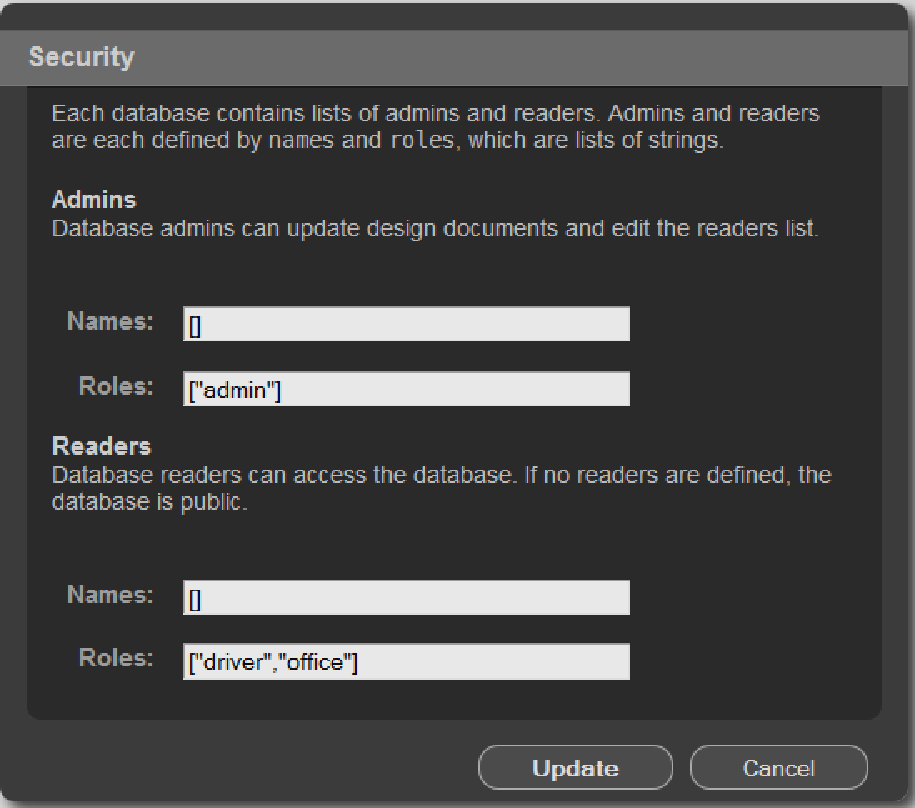
\includegraphics[width=0.8\textwidth]{files/pdf/security.pdf}
	\caption{Admins \& Readers}
	\label{fig:security}
\end{figure}

Auf einer Datenbank können in CouchDB Admins und Readers definiert werden. 
\begin{description}
\item[Admin] Ein Admin hat sämtliche Rechte auf der Datenbank. Er kann die zudem die Datenbank löschen, Designdokumente verändern oder Benutzerrechte ändern.
\item[Reader] Ein Reader hat lesenden und schreibenden Zugriff auf alle Dokumente bis auf die Designdokumente.
\end{description}

\noindent Ein Benutzer kann über 2 verschiedene Arten einer Gruppe zugeordnet werden:
 \begin{itemize}
\item Names: Ein CouchDB-Benutzer muss einen eindeutigen Namen im Format "`org.couchdb.user:[username]"' haben. Die Benutzer werden in einer seperaten Datenbank mit dem Namen "`\_users"' definiert. Wenn der Benutzer dieser Liste (Array aus Strings) hinzugefügt wird, dann besitzt er die entsprechenden Rechte.
\item Roles: Ein Benutzer kann verschiedene Rollen besitzen. Wenn eine seiner Rollen in dieser Liste aufgeführt wird, hat er die entsprechenden Rechte. 
\end{itemize}

\subsection{Rollen in Roadrunner}

Einem Benutzer können keine bis mehrere Rollen zugewiesen werden. Bei jeder Veränderung von Dokumenten auf dem Backendsystem wird von CouchDB eine Benutzerauthentifizierung durchgeführt. Bei dieser Benutzerauthentifizierung wird das Zugriffsrecht auf die Datenbank überprüft und zudem eine Validierung durchgeführt. Bei der Validierung werden alle definierten Validierungsmethoden aufgerufen. Nur wenn alle Validierungen gültig sind wird die gewünschte Änderung an den Dokumenten durchgeführt.
\newline \newline \noindent
Im Projekt Roadrunner wurden 3 verschiedenen Rollen definiert:
\begin{description}
\item[Admin] Ein Admin hat sämtliche Rechte auf der Datenbank. Diese Rollen ist ausschließlich für Administratoren vorgesehen.
\item[Office] Ein Benutzer der Gruppe Office arbeitet mit dem Backendsystem von Roadrunner. Dieser Benutzer arbeitet über die Webapplikation mit Roadrunner.
\item[Driver] Ein Benutzer der Gruppe Driver ist ein Fahrer. Er arbeitet auf dem Androidsystem mit Roadrunner. Auf dem Androidsystem arbeitet er als Admin mit der Datenbank. Eine Einschränkung der Benutzerrechte auf dem Androidsystem ist nicht nötig da die Benutzerauthentifizierung bei der Replizierung der Daten von dem Androidsystem auf das Backendsystem durchgeführt wird. Ein Fahrer kann nur Daten replizieren für die er die entsprechenden Rechte besitzt.
\end{description}

\noindent In den Validierungsmethoden werden die entpsrechenden Rechtevalidierungen durchgeführt. In Tabelle \ref{tab:rechte} sind die Berechtigungen aufgelistet. Ein + bedeutet, dass der Benutzer das Recht besitzt.

\begin{table}
\begin{tabular}{lccc}
& Driver & Office & Admin \\
Benutzerrechte ändern & - & - & + \\
Designdokumente ändern & - & - & + \\
Logeinträge anlegen & + & + & + \\
Logeinträge ändern & - & - & + \\
Logeinträge löschen & - & - & + \\
Andere Dokumente anlegen & - & + & + \\
Andere Dokumente ändern & - & + & + \\
Andere Dokumente löschen & - & + & +
\end{tabular}
\caption{Benutzerrechte}
\label{tab:rechte}
\end{table}

\clearpage
\section{Android Applikation}
\label{sec:android}

Als Hauptsystem in diesem Projekt wurde eine Applikation für die Android
	Plattform erstellt. Diese Applikation dient der mobilen Überwachung
	von Lieferungen bzw. den Gegenständen einer Lieferung.

Android \footnote{http://www.android.com/} ist ein Betriebssystem sowie auch eine Software Plattform für mobile Geräte.
Es werden Smartphones, Netbooks, Mobiltelefone und Tablets unterstützt. Entwickelt wurde das Betriebssystem von der
\emph{Open Handset Alliance} \footnote{http://www.openhandsetalliance.com/}, einem Konsortium von 80 Firmen zur Schaffung offenen Standards 
für mobile Geräte, die von \emph{Google} im Jahr 2007 gegründet wurde (vlg. \cite{OHA07}). 

Wir entschieden uns für Android, da es die gewünschten Anforderungen an unsere mobile Applikation am besten erfüllt. 
Ein wichtiger Aspekt für unsere Entscheidung war, dass Android \emph{Open Source} ist und ständig verbessert wird.
Android unterstützt ebenfalls \emph{CouchDB}, die wir auch in unserem Backend System einsetzen, was ein weiters wichtiges Kriterium war.
Das \emph{Android SDK} ist als Plugin für \emph{Eclipse} \footnote{http://www.eclipse.org/} verfügbar und ermöglichte es uns somit ein 
plattformunabhängige Entwicklung in einer gewohnten Entwicklungsumgebung. Ein weiterer Vorteil von Android ist, dass die Smartphones von
mehreren verschiedenen Herstellern angeboten werden, was dem Kunden einen Gewissen Spielraum bei der Anschaffung der Smartphones gibt.
Ebenfalls war für uns ein einfaches Deployment, mit einfachen Updates, der Anwendung wichtig, welche mittels \emph{adb} und \emph{App-Installer}
ermöglicht wird. Ein Nachteil könnte die fehlerhafte Bedienung des Benutzers sein, die die Funktionsweise der mobilen Applikation beeinträchtigten könnte.

\subsection{Benutzung}

Nach dem sich der Fahrer mit seinem Benutzernamen, seinem Passwort und der ausgewählten Transporteinheit eingeloggt hat, gelangt er auf den \emph{Home} Screen.
Die Benutzeroberfläche des \emph{Home} Screens ist einfach und intuitiv gestaltet. Der Fahrer hat dann die Möglichkeit 
Barcodes zu scannen sowie die Lieferdetails zu den aktuell geladenen Paketen anzusehen.
Nachdem der Barcode eines Pakets gescannt wurde, kann abhängig vom Status des Paketes (aufgeladen - nicht aufgeladen), das Paket
geladen, entladen oder abgeliefert werden. Wenn ein Paket abgeliefert wird, kann der Kunde die Lieferung mit seiner Unterschrift bestätigen.

Mit einem Klick auf den Menüpunkt \emph{My Deliveries} sieht der Fahrer die Adressinformationen des Senders bzw. Empfängers für jede Lieferung.
Weiters können alle Pakete und deren Status einer ausgewählten Lieferung angezeigt werden. 
Außerdem kann die Karte mit der eingezeichnenten Route und der aktuellen Positionen des Fahrers angezeigt werden.

\subsection{Implementierung}

Bei der Implementierung der Benutzeroberfläche wurden bekannte \emph{UI-Patterns} verwendet. Auf dem \emph{Home} Screen der Applikation
wurde das \emph{Dashboard} Pattern verwendet um die Navigation in der Applikation klar und einfach zu gestalten. Des Weitern enthält jeder
Screen eine \emph{Action Bar} im oberen Teil, die dem Benutzer anzeigt in welchem Kontext der Applikation er sich gerade befindet (\emph{breadcrumbs navigation}).
Mit einem Klick auf das \emph{Home} Symbol in der \emph{Action Bar} hat der Benutzer jederzeit die Möglichkeit wieder auf den \emph{Home} Screen zu gelangen.

Die Dienste zur Überwachung der Temperatur und der GPS-Position sowie zum replizieren der Daten mit der serverseitigen Datenbank sind als \emph{Android Services},
die im Hintergrund laufen, implementiert. Somit wird gewährleistet dass diese wichtige Dienste unabhängig von der Applikation, die auch vom Benutzer geschlossen werden kann,
durchgeführt werden. Diese \emph{Android Services} laufen durchgängig im Hintergrund und müssen explizit beendet werden, falls notwendig.

\subsection{Mögliche Erweiterungen}

Mögliche Erweiterungen, die bis jetzt noch nicht umgesetzt wurden, wären beispielsweise eine automatische Berechnung der besten Route, abhängig
von den zu erledigenden Lieferungen. Weiters könnte die berechnete Route in das Navigationssystem \emph{Navigation} von \emph{Google} übernommen werden.
Ein weiterer Nutzen für den Fahrer wäre auch die Darstellung der aktuellen Temperaturwerte seiner geladenen Güter, sowie eine Benachrichtigung wenn diese unter-
bzw. überschritten wird. Eventuell könnte in Zukunft auch eine Benachrichtigung an das Fahrzeug, beispielsweise zum abholen eines Paketes, direkt
aus der Web-Anwendung gesendet werden.



\clearpage
\section{GIT}

\subsection{Unterschiede zu SVN}

\subsection{Arbeitsweise mit GIT}

\subsection{Mögliche Probleme}



\clearpage
\section{Usecases}

\subsection{Login}

Ein Fahrer hat im System einen Benutzer. Durch Benutzername und Passwort kann sich der Fahrer auf dem Android-System einloggen. Als Authentifizierungssystem zum Server werden dabei CouchDB-User verwendet. Details zum Authentifizierungssystem sind unter Abschnitt \ref{security}.

Nach dem Einloggen kann der Fahrer sein Fahrzeug wählen. Das Auswählen des Fahrzeuges ist notwendig, damit das Android-System weiß welche Sensoren auszulesen sind. In Kapitel \ref{sensors} ist beschrieben wie jedes Fahrzeug mit Sensoren ausgestattet wird. 

In Abbildung \ref{fig:login} ist ersichtlich wie der Loginvorgang durchgeführt wird. Nach dem Loginvorgang versucht das System eine Anfrage für neue Daten an den Server zu senden.  Bei einer aktiven Serververbindung werden die Benutzerdaten und das gewählte Fahrzeug an den Server gesendet. Nach einer Authentifizierung des Benutzers wird ermittelt ob für das gewählte Fahrzeug neue Daten bezüglich der Sensoren vorhanden sind. Sind neue Daten vorhanden werden diese per Datenbankreplikation an das mobile Gerät gesendet.

Bei der Replikation werden Container-Dokumente übertragen. In diesen Dokumenten sind die Informationen gespeichert, welche Sensoren auf dem jeweiligen Fahrzeug vorhanden sind und wie diese anzusprechen sind.

\begin{figure}
	\centering
		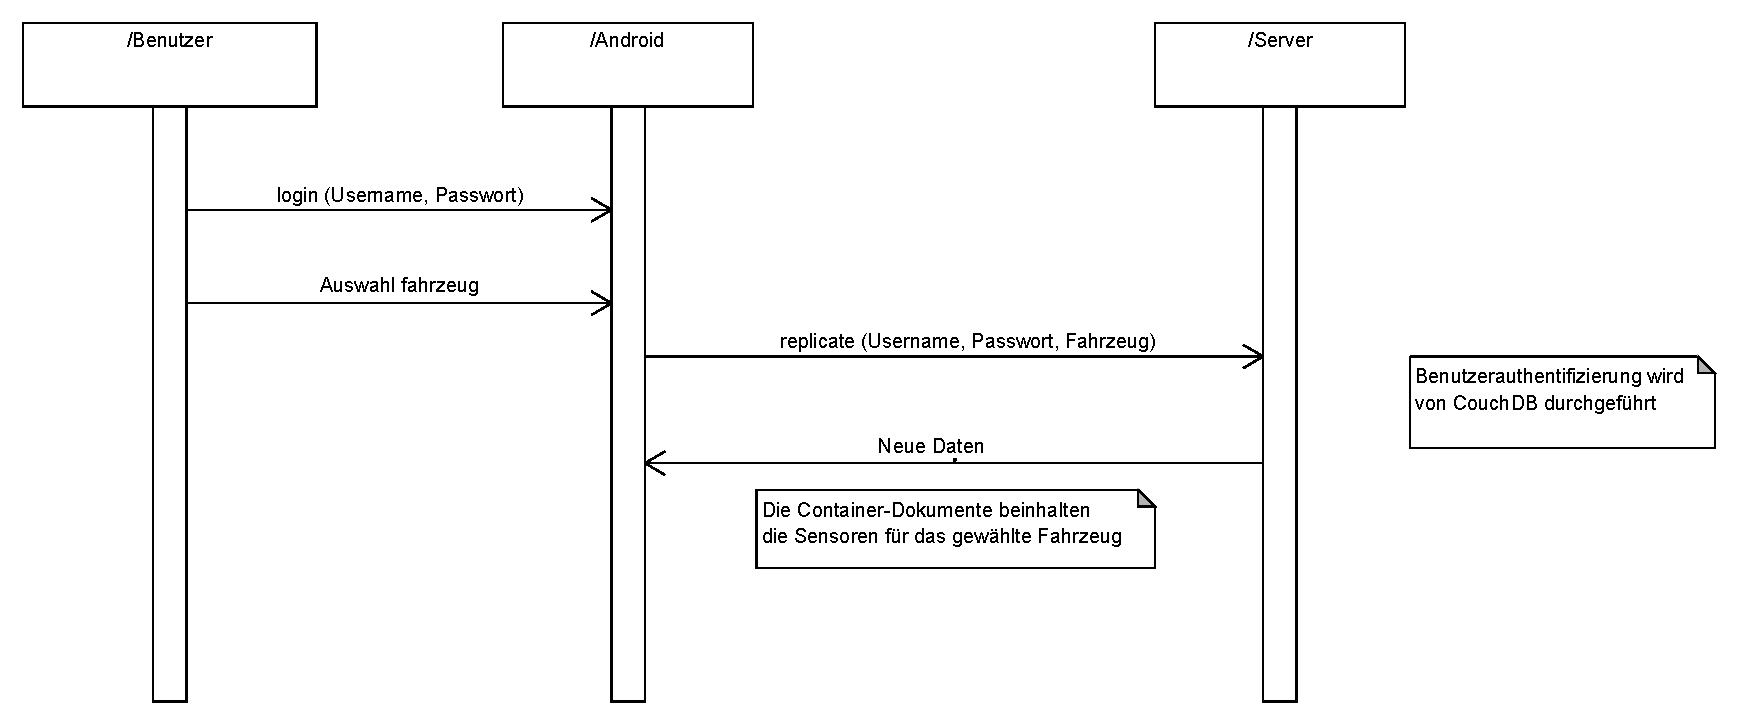
\includegraphics[width=\textwidth]{files/pdf/Login.pdf}
	\caption{Loginvorgang}
	\label{fig:login}
\end{figure}


\begin{itemize}
  \item Wareneingang
  	\subitem registriert Pakete im System
  	\subitem klebt QR-Code auf Pakete

	\item Logister plant und erstellt Lieferungen (neue Auftragsnummer wird
	generiert) \subitem wählt Pakete aus (können mit Sensoren bestückt sein)
		\subitem wählt Fahrer aus 
		\subitem wählt Transportmittel (können mit Sensoren bestückt sein) für
		Lieferungen aus
		\subitem trägt Zielort und Auftraggeber ein
  	
  \item Transporteur
  	\subitem holt oder hat Device mit Roadrunner App
  	\subitem loggt sich im Roadrunner System ein
  		\subsubitem mit Benutzerdaten wird sein/e aktuelle/r Auftrag/Lieferung aufs
  		Device synchronisiert ODER 
  		\subsubitem scannt Pakete und lädt sie in das vom Logistiker ausgwählte
  		Transportmittel
\end{itemize}

\paragraph{Daten-Synchronisierung}
	\textbf{Vorbedingungen: }
	\begin{itemize}
	  \item Transporteur hat sich in der System-App eingeloggt
	\end{itemize}
	
	Die Daten-Synchronisierung oder Replizierung wird durch das Einloggen im
	System angestoßen. Das mobile Gerät erhält folgende Information:
	\begin{itemize}
	  \item Adressen der Sensoren, die das Gerät überwachen sollte
	  \item alle Produkte, Pakete der aktuellen Lieferung, sowie Zielort, etc.
	  \item Überwachungs-Thresholds der Pakete
	\end{itemize}
\par


\clearpage
\input{input/iteration1}

\clearpage
\section{Applikationssicherheit}
\label{sec:security}

\subsection{Zeitsynchronisierung}
\label{subsec:timesync}

In diesem Abschnitt werden Probleme besprochen, die durch fehlerhafte respektive
mangelhaft durchdachte Zeitsynchronisierung oder Verbindungsabbruch entstehen
können.

\paragraph{Problem durch falsche Zeitstempel bei Logeinträgen:}
Betrachtet wird das Szenario ``Umladevorgang eines Produktes''. Das mobile
Gerät der Transporteinheit wird benutzt um den Ausladevorgang aus einem
Container im System zu verarbeiten. Mit dem scannen des Produkts wird auf dem
mobilen Gerät der Transporteinheit ein Logeintrag in dessen lokale Datenbank
erstellt. Genauso wird beim darauffolgenden Ladevorgang der Umladestation ein
Logeintrag auf dessen Gerät erstellt. Wenn das System mit absoluter Zeit
arbeitet und die Uhrzeit des Geräts der Transporteinheit vor jener der
Umladestation ist, dann würde im System der Übernahmevorgang der Umladestation
vor dem Ausladevorgang der Transporteinheit stattfinden.
\par
\paragraph{Lösungsansatz:}
Um dieses Problem zu lösen muss relative Zeit eingeführt und synchronisiert
werden. Für die Zeitsynchronisierung können bekannte Algorithmen für verteilte
Systeme verwendet werden. Mögliche Algorithmen sind Christian's Algorithm oder Berkley Algorithm\footnote{$http://en.wikipedia.org/wiki/Clock_synchronization$}.
\par
Im Projekt Roadrunner wurde Christian's Algorithmus implementiert. Jeder Client misst seine Differenz zur Serverzeit und verwendet diese zur Erzeugung der Zeitstempel. Somit können die unterschiedlichen Uhren bis zu einer gewünschten Genauigkeit synchronisiert werden.

Grundsätzlicher Ablauf zur Ermittlung der Zeitdifferenz ist folgender:
\begin{enumerate}
\item Client erzeugt einen Zeitstempel mit der letzten bekannten Differenz zur Serverzeit.
\item Client sendet eine Anfrage für die Serverzeit an den Server.
\item Server antwortet mit seiner Zeit.
\item Client erzeugt einen zweiten Zeitstempel.
\item Ist die RoundTrip-Zeit klein genug werden die Zeitstempel von Client und Server verglichen.
\item Überschreitet die Zeitdifferenz einen Schwellwert wird auf dem Client die neue Zeitdifferenz gesetzt.
\end{enumerate}

\par
Die Uhren werden bis zu einer gewählten Genauigkeit miteinander synchronisiert. Beim Projekt Roadrunner wurde die Genauigkeit mit 5 Sekunden gewählt. Dies bedeutet, wenn der Client seinen Zeitstempel mit dem von dem Server vergleicht und die Differenz die Genauigkeit überschreitet, dann ermittelt der Client die neue Differenz und verwendet diese zur Erzeugung der nächsten Zeitstempel. Die Synchronisation bis zu einer Genauigkeit von 5 Sekunden wurde gewählt, da ein Umladevorgang sicher länger als 5 Sekunden dauert. Eine zu kleine Genauigkeit hätte zur Folge, dass durch Abweichende RoundTrip-Zeiten ständig die Uhr neu gestellt würde und unnötig viele Zeitsynchronisierungseinträge erstellt würden.
\par
Bei jeder Zeitsynchronisierung wird eine Log-Eintrag für alle geladenene Items erzeugt. Dadurch ist in der History eines Items ersichtlich wann eine Zeitsynchronisierung des Client durchgeführt wurde und welche Log-Einträge einen von der Serverzeit abweichenden Zeitstempel haben.
\par
Bei der Zeitsynchronisierung ist die RoundTrip-Zeit ebenfalls von großer Bedeutung. Ist die RoundTrip-Zeit zu groß wird der Zeitstempel vom Server verworfen und keine Synchronisierung durchgeführt. Nur wenn die RoundTrip-Zeit hinreichend klein ist, kann eine sinnvolle Zeitdifferenz der Zeitstempel ermittelt werden. Für die größte noch erlaubte RoundTrip-Zeit wurde 2 Sekunden gewählt. Dies entspricht etwa der halben Genauigkeit und bei keiner zu großen Netzauslastung sollte ein Request in dieser Zeit auch abarbeitbar sein.

\subsection{Zugriffskontrolle}

Zur Umsetzung des Rechtesystems von Roadrunner werden verschiedene Benutzergruppen eingeführt. Die Rechte werden einerseits direkt auf der Datenbank definiert und zudem noch über Validierungsfunktionen umgesetzt. Die Benutzerauthentifizierung wird von CouchDB durchgeführt.

\subsection{Administratoren \& Benutzer}

\begin{figure}
	\centering
		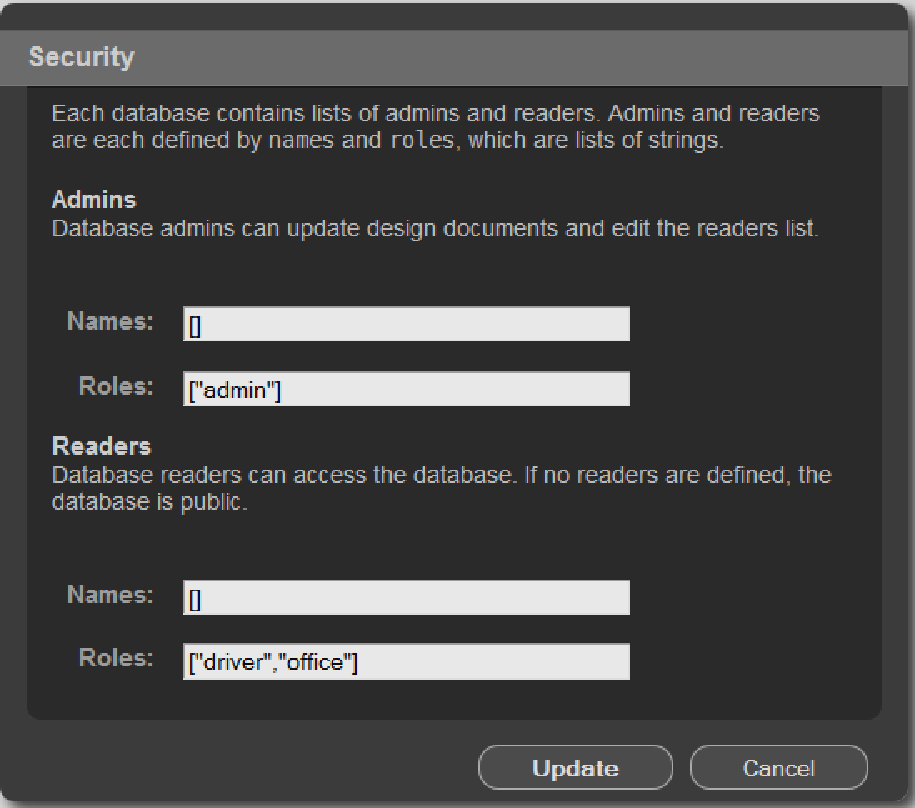
\includegraphics[width=0.8\textwidth]{files/pdf/security.pdf}
	\caption{Admins \& Readers}
	\label{fig:security}
\end{figure}

Auf einer Datenbank können in CouchDB Admins und Readers definiert werden. 
\begin{description}
\item[Admin] Ein Admin hat sämtliche Rechte auf der Datenbank. Er kann die zudem die Datenbank löschen, Designdokumente verändern oder Benutzerrechte ändern.
\item[Reader] Ein Reader hat lesenden und schreibenden Zugriff auf alle Dokumente bis auf die Designdokumente.
\end{description}

\noindent Ein Benutzer kann über 2 verschiedene Arten einer Gruppe zugeordnet werden:
 \begin{itemize}
\item Names: Ein CouchDB-Benutzer muss einen eindeutigen Namen im Format "`org.couchdb.user:[username]"' haben. Die Benutzer werden in einer seperaten Datenbank mit dem Namen "`\_users"' definiert. Wenn der Benutzer dieser Liste (Array aus Strings) hinzugefügt wird, dann besitzt er die entsprechenden Rechte.
\item Roles: Ein Benutzer kann verschiedene Rollen besitzen. Wenn eine seiner Rollen in dieser Liste aufgeführt wird, hat er die entsprechenden Rechte. 
\end{itemize}

\subsubsection{Rollen in Roadrunner}

Einem Benutzer können keine bis mehrere Rollen zugewiesen werden. Bei jeder Veränderung von Dokumenten auf dem Backendsystem wird von CouchDB eine Benutzerauthentifizierung durchgeführt. Bei dieser Benutzerauthentifizierung wird das Zugriffsrecht auf die Datenbank überprüft und zudem eine Validierung durchgeführt. Bei der Validierung werden alle definierten Validierungsmethoden aufgerufen. Nur wenn alle Validierungen gültig sind wird die gewünschte Änderung an den Dokumenten durchgeführt.
\newline \newline \noindent
Im Projekt Roadrunner wurden 3 verschiedenen Rollen definiert:
\begin{description}
\item[Admin] Ein Admin hat sämtliche Rechte auf der Datenbank. Diese Rollen ist ausschließlich für Administratoren vorgesehen.
\item[Office] Ein Benutzer der Gruppe Office arbeitet mit dem Backendsystem von Roadrunner. Dieser Benutzer arbeitet über die Webapplikation mit Roadrunner.
\item[Driver] Ein Benutzer der Gruppe Driver ist ein Fahrer. Er arbeitet auf dem Androidsystem mit Roadrunner. Auf dem Androidsystem arbeitet er als Admin mit der Datenbank. Eine Einschränkung der Benutzerrechte auf dem Androidsystem ist nicht nötig da die Benutzerauthentifizierung bei der Replizierung der Daten von dem Androidsystem auf das Backendsystem durchgeführt wird. Ein Fahrer kann nur Daten replizieren für die er die entsprechenden Rechte besitzt.
\end{description}

\noindent In den Validierungsmethoden werden die entpsrechenden Rechtevalidierungen durchgeführt. In Tabelle \ref{tab:rechte} sind die Berechtigungen aufgelistet. Ein + bedeutet, dass der Benutzer das Recht besitzt.

\begin{table}
\begin{tabular}{lccc}
	& Driver & Office & Admin \\
	Benutzerrechte ändern & - & - & + \\
	Designdokumente ändern & - & - & + \\
	Logeinträge anlegen & + & + & + \\
	Logeinträge ändern & - & - & + \\
	Logeinträge löschen & - & - & + \\
	Andere Dokumente anlegen & - & + & + \\
	Andere Dokumente ändern & - & + & + \\
	Andere Dokumente löschen & - & + & +
\end{tabular}
\caption{Benutzerrechte}
\label{tab:rechte}
\end{table}


\clearpage
\section{Sensorik}\label{sensors}

\subsection{Typen}


\subsection{Wann und wie kommt der Sensor ins System?}

\subsection{Überwachung}

\subsection{Wie werden dem Mobilen Device Sensoren zugeordnet?}

\subsection{Temperatursensoren}
	\paragraph{Hygrosens TLOG20-BLUE}
		Das ist \textit{NICHT} unsere Lösung.
		\url{http://shop.hygrosens.com/Messsysteme-acma/
			Messsysteme-fuer-Temperatur/Temperaturmesssysteme/
			Temperaturmesssysteme-BLUETOOTH/
			BLUETOOTH-Temperaturmesssystem-20-Kanaele.html}
			{hygrosens.com/TLOG20-BLUE, Zugriff am 16.04.2011}
	\par
	
	\paragraph{Ampedrf BT11}
		Das ist \textit{NICHT} unsere Lösung.
		\url{http://www.ampedrf.com/modules.htm}
		{BT11 Class1, Zugriff am 16.04.2011}
		\url{http://www.ampedrf.com/datasheets/BT11_Datasheet.pdf}
		{BT11 Datasheet}
	\par 

	\paragraph{\$149 Programmable Universal Key Fob Sensor}
		Wir haben uns für das BlueRadios BR-FOB-SEN-LE4.0 Device  entschieden, weil es
		eine komplette und etablierte Lösung für Temperatur, Beschleunigungs- und
		Licht-Messung ist.
		\url{http://www.blueradios.com/BR-FOB-SEN-LE4.0-S2A.pdf}
		{Blueradios BR-FOB-SEN-LE4, Zugriff am 16.04.2011}
		
		\url{http://www.blueradios.com/hardware_sensors.htm}
		{Blueradios BR-FOB-SEN-LE4}
	\par

\subsection{Simulation}

Wir haben uns in diesem Projekt entschieden, die Thematik Sensor vollständig zu
simulieren. Einerseits aus zeitlichen Aspekten und andererseits, um unseren
Hauptfokus intensiver ausarbeiten zu können.

\subsection{Wie sieht unsere Sensorsimulation aus?} 

Alle benötigten Sensoren, Zeitsensoren sowie Temperatursensoren werden mit
\emph{nodejs}, wie in Abschnitt~\ref{subsec:nodejs} erläutert, simuliert.


%______________________________________________________________________

\cleardoublepage
\pagenumbering{Roman}

\begin{thebibliography}{99}
\addcontentsline{toc}{section}{Literaturverzeichnis}

\bibitem[Gamma 94]{Gamma94}
  E.\ Gamma, R.\ Helm, R.\ Johnson, J.\ Vlissides:
    Design Patterns: Elements of Reusable Object-Oriented Software.
	MA: Addison-Wesley, 1994.

%    Web-References
%______________________________________________________________________

\hspace{-\leftmargin}{\Large\bfseries Web-Referenzen} % Wüster Hack %-|

\bibitem[Wikipedia 10a]{Wikipedia10a}
  Wikipedia: Node.js
    \url{http://de.wikipedia.org/wiki/Node.js}, besucht am 20.04.2011.

\end{thebibliography}


% ende des hauptteils
\fancyhead[R]{} % Keine Kopfzeile mehr oben auf jeder Seite

\end{document}
